\documentclass[10pt,nofootinbib,letterpaper]{revtex4}
%\usepackage[nocap]{ctex}

\usepackage{xeCJK}
% if \usrpackage{xetex} it will invoke the open source Fandol Song Font by default, which lack many Chinese characters
% Linux Requires TrueType Fonts from Windows (locating at C:\Windows\Fonts), and Simlink 
% ln -s blablabla /usr/share/fonts/WindowsFonts 
\setCJKmainfont[BoldFont={SimHei},ItalicFont={KaiTi}]{SimSun}
\setCJKfamilyfont{kaishu}{KaiTi} 
\newcommand*{\kaishu}{\CJKfamily{kaishu}}


\usepackage{amsmath,amssymb,amsfonts,mathrsfs,bm,dsfont}
\usepackage{slashed}
\usepackage{enumerate}
\usepackage{enumitem} % Customize itemize, see https://ctan.org/tex-archive/macros/latex/contrib/enumitem/
\usepackage[all]{xy}
\usepackage[noabbrev]{cleveref} % multiple equation ref, see https://tex.stackexchange.com/questions/314217/how-i-can-refer-multiple-equation-in-latex?rq=1
\usepackage[normalem]{ulem}	% delete line
\usepackage{array}
\usepackage{graphics,color}
\usepackage{tikz}
	\usetikzlibrary{calc}
	\usetikzlibrary{decorations.markings}
	\usetikzlibrary{arrows}
	\usetikzlibrary{patterns}
	%\usetikzlibrary{shapes.callouts}
\tikzset{
    level/.style = {
        ultra thick,
        blue,
    },
    connect/.style = {
        dashed,
        red
    },
    label/.style = {
        text width=2cm
    }
}
\usepackage{pgfplots}
%\usepackage[citestyle=authortitle]{biblatex} % able to cite the title, author and year
%\usepackage{hyperref}
\usepackage{feynmp} % feymann diagram
\usepackage{extarrows}
\usepackage[normalem]{ulem} % 文字划掉(横),与 cite 兼容问题,见 https://tex.stackexchange.com/questions/98222/ulem-incompatibility-with-multiple-entries-in-cite

\newcommand*\dd{\mathop{}\!\mathrm{d}}
\newcounter{Claim}[section]
\newenvironment{Claim}[1][]{{\par\normalfont\bfseries \underline{Claim~\stepcounter{Claim}\arabic{Claim}.}~#1~~}}{\par}
\newcounter{Proposition}[section]
\newenvironment{Proposition}[1][]{{\par\normalfont\bfseries \underline{Proposition~\stepcounter{Proposition}\arabic{Proposition}.}~#1~~}}{\par}
\newcounter{Note}[section]
\newenvironment{Note}[1][]{{\par\normalfont\bfseries \underline{Note~\stepcounter{Note}\arabic{Note}.}~#1~~}}{\par}
\newcounter{Lemma}[section]
\newenvironment{Lemma}[1][]{{\par\normalfont\bfseries \underline{Lemma~\stepcounter{Lemma}\arabic{Lemma}.}~#1~~}}{\par}
\newcounter{Corollary}[section]
\newenvironment{Corollary}[1][]{{\par\normalfont\bfseries \underline{Corollary~\stepcounter{Corollary}\arabic{Corollary}.}~#1~~}}{\par}
\newenvironment{Proof}{{\par~{\normalfont\bfseries $\vartriangleright$}~~}}{\hfill $\square$\par\hfill\par} %\par
\newcounter{Def}[section]
\newenvironment{Def}[1][]{{\par\normalfont\bfseries \underline{Definition~\stepcounter{Def}\arabic{Def}.}~#1~~}}{\par}
\newcounter{Assumption}[section]
\newenvironment{Assumption}[1][]{{\par\normalfont\bfseries \underline{Assumption~\stepcounter{Assumption}\arabic{Assumption}.}~#1~~}}{\par}



\allowdisplaybreaks[4] %允许 align 跨页编排

%\def\checkmark{\tikz\fill[scale=0.4](0,.35) -- (.25,0) -- (1,.7) -- (.25,.15) -- cycle;}
%\def\G{\mathcal{G}}
\def\Z{\mathcal{Z}}
\def\H{\mathcal{H}}
\def\D{\mathcal{D}}

\begin{document}
\title{Effective Field Theory for Hall Viscosity}
\author{Xiaodong Hu}
%\altaffiliation[Also at ]{Boson College}
\email{xiaodong.hu@bc.edu}
\affiliation{Department of Physics, Boston College}

\date{January 7, 2021}

\begin{abstract}
	Hall viscosity, by definition, is related to the stress response of the system to the perturbation of the metric \cite{avron1995viscosity,bradlyn2012kubo}. In this note, however, we will follow the work of Hoyos and Son \cite{hoyos2012hall} to show that Hall viscosity also appears in pure electromagnetic reponse of finite wave vector in any system with equal charge/mass ratio and Galilean invariance.\par
	%\begin{center}
		\hfill\par
		{\centering\kaishu 致虚极,守静笃。万物并作,吾以观其复。\\[0.5em]}
	%\end{center}
	\hfill------ 老子「道德经」
\end{abstract}

\maketitle
\tableofcontents


\section{Motivation: Physical Argument}
	To the lowest order approximation (of wave vector), the velocity of an electron in a plane with external electrical field along $x$ direction $\bm{E}=E_x\hat{x}$ and magnetic field piercing throught the plane $\bm{B}\equiv B\hat{z}$ satisfies
	\begin{equation}\label{1.1.1}
		q(v_yB+E_x)=0.
	\end{equation}
	If we turn on the $x$-dependence of the scalar potential $E_x(x)=-\partial_x\phi(x)$, as is illustrated in FIG. \ref{Fig:flow},
	\begin{figure}[!htp]
		\centering
		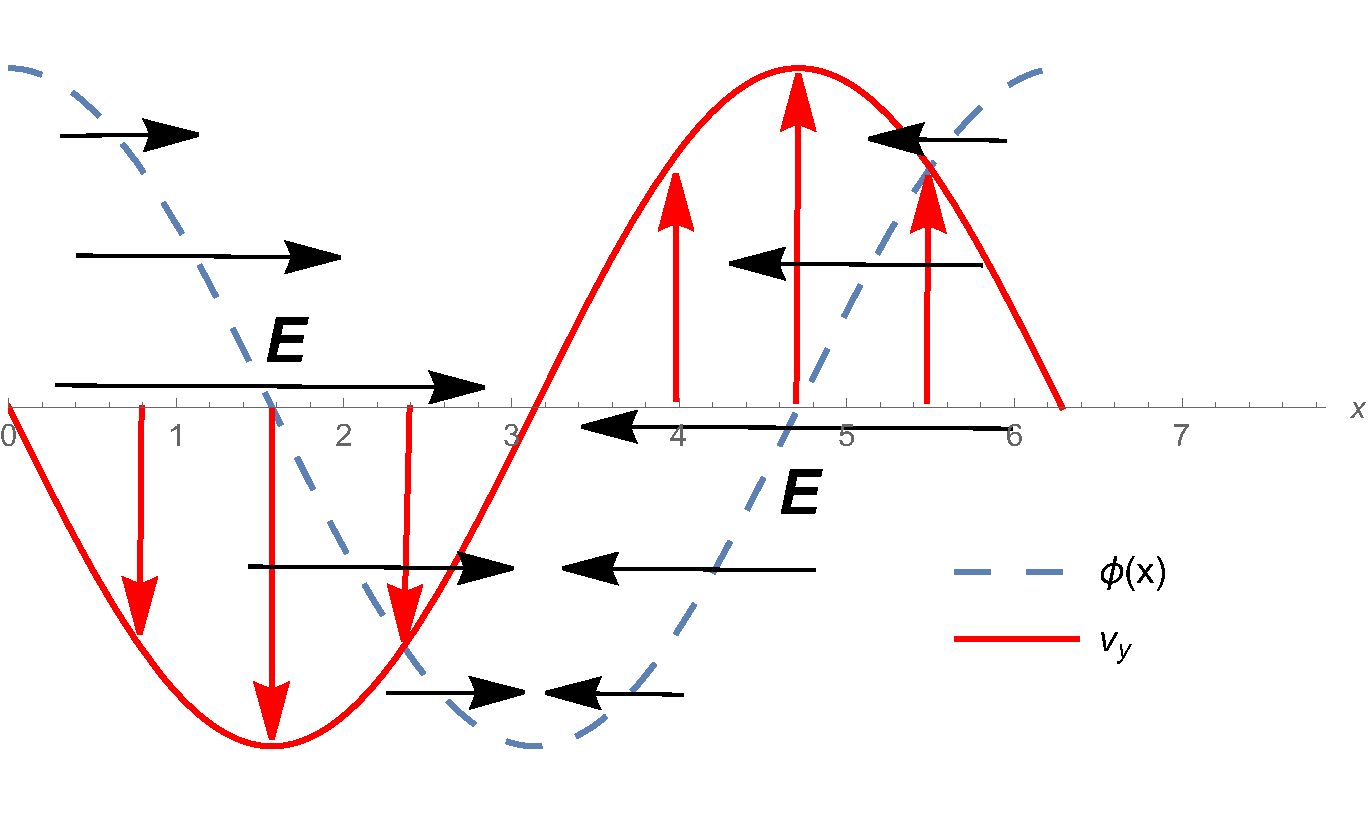
\includegraphics[scale=0.4]{Flow.pdf}
		\caption{An example of inhomogeneous $E_x$ distribution and $v_y$ distribution along $x$-direction.}
		\label{Fig:flow}
	\end{figure}
	then \textbf{the shear flow (fluctuating $v_y(x)$ distribution) will give a nonzero strain rate, which, in turn leads to an additional stress with the existence of Hall viscosity\footnote{Recall the adiabatic interpretation of the Hall viscosity $\sigma_{\alpha\beta}\equiv\lambda_{\alpha\beta\gamma\delta}u^{\gamma\delta}-\eta_{\alpha\beta\gamma\delta}\dot{u}^{\gamma\delta}$}. Such extra force will modify the original force balance condition, inducing a correction to the charge current along $y$-direction, i.e., the finite-$q$ correction of the electromagnetic response}.\par
	More precisely, the strain rate $\dot{u}^{xy}=\dot{u}^{yx}=\frac12(\frac{\partial\dot{u}^y}{\partial x}+\frac{\partial\dot{u}^x}{\partial y})=\frac12 \partial_x v_y$, induces through Hall viscosity $\eta^A=\eta_{xxxy}=\eta_{xxyx}$ a correction to the stress $\sigma_{xx}=-\eta_{xxxy}\dot{u}^{xy}-\eta_{xxyx}\dot{u}^{yx}=-2\eta^A\dot{u}^{xy}$. Therefore, there will be a correction to the force along $x$-direction (since $\sigma^{xy}=0$)
	\begin{equation*}
		f_x=-\partial_x\sigma^{xx}=2\eta^A \partial_x\dot{u}^{xy}=\eta^A \partial_x^2v_y(x).
	\end{equation*}
	And the force balance condition becomes
	\begin{equation}\label{1.1.2}
		q(v_y(x)B+E_x(x))+f_x[v_y(x)]=0.
	\end{equation}
	Inserting the zeroth-order expression of $v_y$ in \eqref{1.1.1}, we get the first-order correction to the velocity $\Delta v_y$, and the correction to the charge current
	\begin{equation*}
		\Delta j_y=q\Delta v_y=-\dfrac{f_x}{B}=-\dfrac{\eta^A}{B^2}\partial_x^2 E_x(x).
	\end{equation*}
	Thus the first-order correction to transverse conductivity reads
	\begin{equation}\label{1.1.3}
		\sigma_{xy}^{(1)}(q)=\dfrac{\eta^A}{B^2}q^2.
	\end{equation}

	However, the first-order correction to the current not only comes from the extra stress, but also the extra fluctuation of the magnetization $\Delta\bm{j}=\hat{z}\times\nabla\delta\bm{M}$. This is because the curl of the velocity field $\frac12 \partial_xv_y$ can also be interpreted as a local angular velocity field
	\begin{equation*}
		\Omega(x)\equiv\dfrac{1}{2}\partial_x v_y=-\dfrac{1}{2B}\partial_x E_x(x).
	\end{equation*}
	Namely \textbf{the lab frame is relatively rotating with the quantum fluids in the angular velocity $\Omega(x)$. By anology of the Coriolis force and Lorentz force\footnote{Coriolis force $\bm{F}=e\bm{v}\times\bm{B}$; Lorentz force $\bm{F}=q\bm{v}\times B$.}, in the frame of fluids there is an extra local fluctuation of the magnetic field $\delta B=2m\Omega/e$ through inhomogeniety of $E_x(x)$}. Because quantum Hall fluid is a diamagnetic material, given the $B$-dependent energy density the magnetization reads $M=-\partial \varepsilon/\partial B$. Magnetization is a constant in the usual case. However, due to the fluctuation of the effective magnetic field, we have
	\begin{equation*}
		\delta M=-\dfrac{\partial^2 \varepsilon}{\partial B^2}\delta B=\varepsilon''(B)\dfrac{m}{eB}\partial_x E_x.
	\end{equation*}
	And the additional correction to the transverse current is
	\begin{equation*}
		\Delta j_y=\hat{z}\times \partial_x(\delta M)=\varepsilon''(B)\dfrac{m}{eB}\partial_x^2 E_x,
	\end{equation*}
	giving
	\begin{equation}\label{1.1.4}
		\sigma^{(2)}_{xy}(q)=-\dfrac{m \varepsilon''(B)}{eB}q^2.
	\end{equation}
	Combining \eqref{1.1.3} and \eqref{1.1.4}, we get the main results
	\begin{equation}\label{1.1.5}
		{\color{red}\dfrac{\sigma_{xy}(q)}{\sigma_{xy}(0)}=1+\bigg[\dfrac{\eta^A}{n\hbar}-\dfrac{2\pi}{\nu}\dfrac{\ell^2}{\hbar\omega_c}B^2 \varepsilon''(B)\bigg](q\ell)^2+\mathcal{O}((q\ell)^4)}.
	\end{equation}
	Read shows \cite{read2009non} that the Hall viscosity $\eta^A=\frac{1}{2}n\bar{s}\hbar$ so the first part in the square bracket is \emph{universal}. As for the second part (which is clearly system-depent), its magnitude can be obtained by exerting external magnetic fluctuations $\delta B_{\text{ext}}$. The logic is the same as we have shown above. Thus \textbf{\color{red}measurable finit-$q$ dependence of the Hall conductivity does give the Hall viscosity}.

\section{Effective Field Theory of Quantum Hall Fluids}
	In this section, we will prove that the two parts in the square bracket of \eqref{1.1.5} is fixed by the symmetry-allowed effective field theory (even with their coefficients).

	\subsection{Non-relativistic General Coordinate Transformation}
		\textbf{The general rules to write down an effective field theory is by power counting and listing all symmetry allowed terms with some unknown coefficients}. However, there is one more requirement that is naturally satisfied in relativistic EFT so may be frequently omitted in the other cases --- the \emph{special/general covariance principle}, or \emph{diffeomorphism covariance}, stating that \textbf{\color{red}the form of physical laws (or in EFT the form of action) remains unchanged under any general coordinate transformation}. For example, a relativistic theory of free massive bosonic complex scalar field in (curved) $(3+1)$-D spacetime $M$ have the action
		\begin{equation}\label{2.1.1}
			S=-\int\dd^4x\,\sqrt{-g}(g^{\mu\nu}\partial_\mu\Psi^* \partial^\mu\Psi+m^2c^2|\Psi|^2).
		\end{equation}
		Taking the bosonic field operator $\Psi$ as the scalar field on the manifold $\Psi:M\to\mathbb{R}$, then as a scalar, the action is certainly invariant under general transformation $x^\mu\mapsto {x'}^\mu$:
		\begin{equation*}
			\Psi(x)\to\Psi(x'),\quad g_{\mu\nu}(x)\to g'_{\mu\nu}(x')\equiv\dfrac{\partial x^\rho}{\partial{x'}^\mu}\dfrac{\partial x\sigma}{\partial{x'}^\nu}g_{\rho\sigma}(x(x')),
		\end{equation*}
		or infinitesimally ${x'}^\mu=x^\mu+\xi^\mu$ such that
		\begin{equation}\label{2.1.2}
			\delta\Psi=-\xi^\lambda \partial_\lambda\Psi,\quad \delta g_{\mu\nu}=-\xi^\lambda \partial_\lambda g_{\mu\nu}-g_{\lambda\nu}\partial_\mu\xi^\lambda-g_{\mu\lambda}\partial_\nu\xi^\lambda.
		\end{equation}
		Interacting terms of higher orders should also satisfy such diffeomorphism invariance \eqref{2.1.2}.
		\begin{center}
			$\ast$~$\ast$~$\ast$
		\end{center}\par
		Now if we switch to consider the non-relativistic EFT of a free \emph{massive}\footnote{For massless Dirac fermion, things get more complicated. The problem is, the Dirac spinor are the basis of the \emph{half-integer} spinor representation of $\mathfrak{sl}(2,\mathbb{C})$. They cannot be constructed from \emph{any} tensor representations (of \emph{integer} highest weight). However, in GR covariance principle requires all physical object being tensor fields. Thus we have to use viebein formalism to making GR a gauge theory as well. See my writing notes.} boson/fermion coupling with external $U(1)$ gauge field in $(3+1)$-D
		\begin{equation}\label{2.1.3}
			S=\int\dd t\dd\bm{x}\sqrt{g}\bigg[\dfrac{i}{2}\psi^\dagger\overset{\leftrightarrow}{\partial_t}\psi-A_0\psi^\dagger\psi-\dfrac{g^{ij}}{2m}(\partial_i\psi^\dagger-iA_i\psi^\dagger)(\partial_j\psi-iA_j\psi)\bigg],
		\end{equation}
		then with the same reason, besides of the familiar local $U(1)$ gauge invariance
		\begin{equation*}
			\psi\to\psi'=e^{i\alpha}\psi,\quad A_0\to A_0'=A_0-\dot{\alpha},\quad A_i\to A_i'=A_i-\partial_i\alpha_i,
		\end{equation*}
		there should be an extra diffeomorphism invariance under $x^i\to{x'}^i$  for the spatial part of the action
		\begin{equation*}
			\psi(t,\bm{x})\to\psi(t,\bm{x'}),\quad A_0(t,\bm{x})\to A_0(t,\bm{x'}),\quad A_i(t,\bm{x})\to A_i(t,\bm{x'}),\quad g_{ij}(t,\bm{x})\to g'_{ij}(t,\bm{x'})=\dfrac{\partial x^k}{\partial{x'}^i}\dfrac{\partial x^\ell}{\partial{x'}^j}g_{kl}(t,\bm{x}(\bm{x'})),
		\end{equation*}
		or infinitesimally
		\begin{subequations}
			\begin{align}
				\delta\psi&=i\alpha\psi-\xi^k \partial_k\psi,\label{2.1.4a}\\
				\delta A_0&=-\dot{\alpha}-\xi^k\partial_k A_0,\label{2.1.4b}\\
				\delta A_i&=-\partial_i \alpha-\xi^k \partial_k A_i-A_k \partial_i\xi^k,\label{2.1.4c}\\
				\delta g_{ij}&=-\xi^k\partial_k g_{ij}-g_{ik}\partial_j\xi^k-g_{kj}\partial_i\xi^k.\label{2.1.4d}
			\end{align}
		\end{subequations}
		Direct calculation shows that action \eqref{2.1.3} is indeed invariant under \cref{2.1.4a,2.1.4b,2.1.4c,2.1.4d}, providing that spatial variation is \emph{time-independent} $\xi^i=\xi^i(\bm{x})$.\par
		However, the spatial part of the action keeps to be a scalar no matter $\xi^i$ depends on time or not (as a contrast, the $U(1)$ phase depends both on space and time $\alpha=\alpha(t,\bm{x})$). Hence we expect the diffeomorphism invariance also applies to \emph{time-dependent} spatial variations $\xi^i=\xi^i(t,\bm{x})$. This time, the action will acquire a residual term under the above infinitesimal transformations \cref{2.1.4a,2.1.4b,2.1.4c,2.1.4d}
		\begin{equation}\label{2.1.5}
			\delta S=-\dfrac{i}{2}\int\dd t\dd\bm{x}\,\dot{\xi}^k\psi^\dagger\overset{\leftrightarrow}{\partial_k}\psi.
		\end{equation}
		That is to say, to keep the diffeomorphism invariance for general $\alpha(t,\bm{x})$ and $\xi^i(t,\bm{x})$, we have to modify the infinitesimal transformation to the so-called \emph{non-relativistic general coordinate transformations} \cite{son2006general}
		\begin{subequations}
			\begin{align}
				\delta\psi&=i\alpha\psi-\xi^k \partial_k\psi,\label{2.1.6a}\\
				\delta A_0&=-\dot{\alpha}-\xi^k\partial_k A_0{\color{red}-A_k\dot{\xi}^k},\label{2.1.6b}\\
				\delta A_i&=-\partial_i \alpha-\xi^k \partial_k A_i-A_k \partial_i\xi^k{\color{red}+mg_{ik}\dot{\xi}^k},\label{2.1.6c}\\
				\delta g_{ij}&=-\xi^k\partial_k g_{ij}-g_{ik}\partial_j\xi^k-g_{kj}\partial_i\xi^k.\label{2.1.6d}
			\end{align}
		\end{subequations}
		The Galilean invariance on \emph{flat} space $g_{ij}=\delta_{ij}$ can be seen by particular choice of $\alpha=mv_ix^i$ and $\xi^i=v^it$, giving
		\begin{align*}
			\psi(t,\bm{x})&\to\psi'(t,\bm{x})=e^{im\bm{v\cdot x}}\psi(t,\bm{x}-\bm{v}t),\\
			A_0(t,\bm{x})&\to A_0'(t,\bm{x})=A_0(t,\bm{x}-\bm{v}t)-\bm{v}\cdot\bm{A}(t,\bm{x}-\bm{v}t),\\
			\bm{A}(t,\bm{x})&\to\bm{A'}(t,\bm{x})=\bm{A}(t,\bm{x}-\bm{v}t).
		\end{align*}
		So what we have done in \cref{2.1.6a,2.1.6b,2.1.6c,2.1.6d} is actually \textbf{one (natural) way of gauging the non-relativistic translation symmetry and Galilean symmetry of the flat space to the curved background}. And the ``naturality'' can be seen from the \emph{Kaluza-Klein reduction} of the relativistic diffoemorphism transformation by taking the limit $c\to\infty$. Please refer to the section 3.2 of \cite{son2006general} for details.

	\subsection{Wen-Zee Term of Quantum Hall Fluids}
		The lowest-order bulk effective action of FQHE on a \emph{flat} space is known to be
		\begin{equation}\label{2.2.1}
			S[a_\mu,A_\mu]=\int\dd^3x\,\left(\dfrac{\nu}{4\pi}\varepsilon^{\mu\nu\rho}a_\mu \partial_\nu a_\rho-\dfrac{e}{2\pi}\varepsilon^{\mu\nu\rho}A_\mu \partial_\nu a_\rho\right),
		\end{equation}
		where $a_\mu$ is called the hydrodynamic\footnote{Wen construct the ``hydrodynamic'' theory in \cite{wen1992classification,wen1995topological} of bulk FQH fluids by assuming the action to be local functional of the conserved currents $S[J_\mu]$. But this is more like writing down an effective field theory but NOT the standard hydrodynamic theory. In modern hydrodynamic theory we construct the conserved quantities with hydrodynamic variables by the second law of thermodynamics.} gauge field of the local conserved current $J^\mu\equiv\frac{1}{2\pi}\varepsilon^{\mu\nu\rho}\partial_\nu a_\rho$ such that $\partial_\mu J^\mu\equiv0$. Integration of the hydrodynamic fields leads to the induced action of external gauge fields, that expresses the Chern-Simons type response to the electromagneitc background
		\begin{equation}\label{2.2.2}
			S_{\text{eff}}[A_\mu]=\dfrac{\nu}{4\pi}\int A\wedge\dd A.
		\end{equation}

		\indent The filling factor $\nu$  (an integer from quantization) is usuall related with the number of electrons $N_e$ and number of fluxes $N_\phi$ by $\nu\equiv N_e/N_\phi$. However, it was observed by Haldane early in 1983 in \cite{haldane1983fractional} that the Laughlin function for the fully-filled LLL $\nu=1$ on a \emph{spherical geometry} has $2S+1=N_e$ degeneracy\footnote{It is because the Hamiltonian has $\mathfrak{su}(2)$ symmetry, so the Laughlin function also furnishes as the representation of $\mathfrak{su}(2)$ Lie algebra, which is labeled by its highest weight (angular momentum) $S$ and has $2S+1$ degeneracy.}, while Dirac quantization condition demands $2S=N_\phi$. Thus on a sphere we have
		\begin{equation}\label{2.2.3}
			N_\phi=\nu^{-1}N_e+\mathcal{S}
		\end{equation}
		with the (Wen-Zee) shift $\mathcal{S}=1$. Similarly, if the only the \emph{second} Landau level is fully-filled $\nu=1$, the degeneracy is increased to $2S+3=N_e$ while the Dirac quantization condition $2S=N_\phi$ remains unchanged. So in this case we have rather $\mathcal{S}=3$.\par
		Such weird shift does not come into the view of the mainstream untile Wen and Zee developed the general effective field theory of the abelian FQH fluid \cite{wen1992classification} (with arbitrary orders of virtual excitation of quasiparticles/quasiholes and residual physical excitation of quasiparticles/quasiholes)
		\begin{equation}\label{2.2.4}
			\mathcal{L}[a_\mu^I,A_\mu,j_{\text{qp}}]=-\dfrac{1}{4\pi}K_{IJ}\varepsilon^{\varepsilon\nu\rho}a_\mu^I \partial_\nu a_\rho^J-\dfrac{1}{2\pi}t_I \varepsilon^{\mu\nu\rho}A_\mu \partial_\nu a_\rho^I+j_{qp}^\mu\ell_I a_\mu^I.
		\end{equation}
		They noticed that if EFT \eqref{2.2.4} is used to describe the ground state of fully-filled lowest and second LL on a sphere, they should have the same $K$-matrix $K_{11}=1$, charge vector $t_I=(1,0)^T$, and vector $\ell_I=\mathbf{0}$. Thus \textbf{the effective field theory \eqref{2.2.4} still does not provide a complete description of the QH liquids}.\par
		So how to improve this? The answer is almost straight forward: recall that \eqref{2.2.4} is constructed without any information of the background, so we must miss some relevant terms describing the coupling with the geometry. And because the original EFT is written in terms of hydrodynamic gauge fields, it is also helpful to formulate the general relativity as a gauge theory for a unified description. More specifically, given a tagent bundle $TM$ (or more general a tensor bundle $T^r_s(M)$) with the base manifold equipped with a metric structure, there is a canonical choice of the basis of each tagent space $T_pM$ from the basis $\{\partial/\partial x^\mu\}$ by a proper orientation-preserving rotation $e_a\equiv e_a^{~\mu}\frac{\partial }{\partial x^\mu}$ for $e_a^{~\mu}\in\mathrm{GL}(n,\mathbb{K})$ such that
		\begin{equation*}
			e_a^{~\mu}e_b^{~\nu}g_{\mu\nu}\equiv\delta_{ab}.
		\end{equation*}
		The LHS is just inner produce of two basis $\langle e_a,e_b\rangle\equiv g(e_a,e_b)=e_a^{~\mu}e_b^{~\nu}g_{\mu\nu}$, so we are actually working on a \emph{orthogonal frame bundle} with the gauge group $O(n)$.\par
		For the special three-dimensional \emph{non-relativistic} product manifold where time is isolated $M=\mathbb{R}\times N$, the metric is only curved on the \emph{spatial} manifold $N$ (while keeping vanishing for space-time and time-time components $g_{00}=g_{0i}=0$), so are the local invertible rotation
		\begin{equation}\label{2.2.5}
			e_a^{~i}e_b^{~j}g_{ij}\equiv\delta_{ab}.
		\end{equation}
		For those non-invertible matrix, we can simply assume that $e_A^{~\mu}$ and $e^A_{~\mu}$ vanishes for all space-time, time-space and time-time components ($\mu=0,1,2$ and $A=0,1,2$).\par
		Now that the structure group is $O(2)\simeq U(1)$, we can treat the hydrodynamic gauge field $a\equiv a_\mu\dd x^\mu$ and the (matrix-valued) connection $1$-from $\omega^a_{~b}\equiv\omega_{\mu~b}^{~a}\dd x^\mu$ of the frame bundle in a unified way. The latter one can be determined from Cartan's first structure equation (for torsion free manifold)
		\begin{equation*}
			\dd e+\omega\wedge e=0,
		\end{equation*}
		or in space-time components $\partial_\mu e^A_{~\nu}+\omega_{\mu~B}^{~A}e^B_{~\nu}=0$. After contraction with $e^C_{~\lambda}\delta_{BC}$ and $g^{\nu\lambda}$, we get
		\begin{equation*}
			\omega_{\mu AB}=\dfrac{1}{2}\partial_\mu e_{A\lambda}\cdot e_B^{~\lambda},
		\end{equation*}
		which is antisymmetric in the last two subsripts $\omega_{\mu AB}\equiv-\omega_{\mu BA}$ since $e_{A\lambda}e_B^{~\lambda}\equiv\delta_{AB}$.\par
		Denoting $\omega_\mu^C\equiv\frac{1}{2}\varepsilon^{ABC}\omega_{\mu AB}$, then
		\begin{equation*}
			\omega_\mu^a\equiv\dfrac{1}{2}\varepsilon^{b0a}\omega_{\mu b0}=\dfrac{1}{4}\varepsilon^{b0a}e_0^{~\lambda}\partial_\mu e_{b\lambda}\equiv0,\quad a=1,2,
		\end{equation*}
		because $e_0^{~\lambda}\equiv0$ by construction. While
		\begin{equation*}
			\omega_0\equiv\omega_0^0=\dfrac{1}{2}\varepsilon^{ab}e^{aj}\partial_0e_j^{~b},\quad\omega_i\equiv\omega_i^0=\dfrac{1}{2}(\varepsilon^{ab}e^{aj}\partial_i e_j^b- \varepsilon^{jk}\partial_j g_{ik}).
		\end{equation*}
		\indent Before using $a_\mu$ and $\omega_\mu$ to construct the EFT of quantum Hall fluids on a curved background, we have to specify the power counting of our theory. \textbf{There is an ambiguity in choosing the counting scheme because the time derivative and spatial derivative can in principle have different powers of the expansion parameter}. For definiteness, we will demand all quantities proportional to the power of the small\footnote{For example, in FQHE of filling $\nu<1$, we have $\varepsilon(B)=\frac{\nu}{4\pi}\frac{\hbar\omega_c}{\ell^2}$.} energy density $\varepsilon(B)$, times power of cyclotron frequency $\omega_c$ and magnetic length $\ell$. All external fields vary slowly in space and time, but in different order
		\begin{equation*}
			\partial_0\sim \varepsilon^2\omega_c, \quad\partial_i\sim \varepsilon\ell^{-1}.
		\end{equation*}
		And the magnitude of external perturbation to be
		\begin{equation*}
			\delta A_0\sim \varepsilon^0\omega_c,\quad\delta A_i\sim \varepsilon^{-1}\ell^{-1},\quad \delta g_{ij}\sim \varepsilon^0
		\end{equation*}
		such that the variation of potential $A_0\sim\mathcal{O}(1)$, magnetic field $B=\varepsilon^{ab}\partial_a A_b\equiv\varepsilon^{ij}\partial_i A_j/\sqrt{g}\sim\mathcal{O}(1)$, and the metric $\delta g_{ij}\sim\mathcal{O}(1)$ are allowed, while the electric field is small $E_i=\partial_i A_0- \partial_0 A_i\sim\mathcal{O}(\varepsilon)$. Under this scheme, the Chern-Simons action \eqref{2.2.2} is of order $\mathcal{O}(1)$. And the spin connection is of order $\omega_\mu\sim\mathcal{O}(\varepsilon^2)$ from \eqref{2.2.5}.\par
		Since $\omega_\mu$ has the same role as $A_\mu$, we can safely write down the most relevant terms for EFT (called Wen-Zee term)
		\begin{equation}\label{2.2.6}
			S_{\text{WZ}}=\dfrac{k}{2\pi}\int\dd^3x\,\varepsilon^{\mu\nu\rho}\omega_\mu \partial_\nu A_\rho,
		\end{equation}
		and
		\begin{equation}\label{2.2.7}
			S_{\text{Grav. C-S}}=c\int\dd^3\,\varepsilon^{\mu\nu\rho}\omega_\mu \partial_\nu \omega_\rho.
		\end{equation}
		However, $S_{\text{Grav. C-S}}$ is of order $\mathcal{O}(\varepsilon^4)$ so will not be considered in this letter.\par
		The Riemann curvature tensor can be obtained from the Cartan's second structure equation
		\begin{equation*}
			\dd\omega^a_{~b}+\omega^a_{~c}\wedge\omega^c_{~b}=R^a_{~b},
		\end{equation*}
		giving the Ricci tensor
		\begin{equation*}
			R^{ab}_{ij}=(\partial_i\omega_j-\partial_j\omega_i)\varepsilon^{ab}\implies R=2\dfrac{\varepsilon^{ij}\partial_i\omega_j}{\sqrt{g}}.
		\end{equation*}
		So Wen-Zee term can be re-arranged into
		\begin{equation}\label{2.2.8}
			S_{\text{WZ}}=\dfrac{k}{2\pi}\int\dd^3x\left(\dfrac{\sqrt{g}}{2}A_0R+\varepsilon^{ij}\dot{A}_i\omega_j+\sqrt{g}B\omega_0\right).
		\end{equation}
		Together with the electromagnetic Chern-Simons action \eqref{2.2.2}, then the total number of electron is (collecting terms coupling with $A_0$)
		\begin{equation}\label{2.2.9}
			N_e\equiv\int\dd^2x\sqrt{g}J_0=\int\dd^2x\sqrt{g}\left(\dfrac{\nu}{2\pi}B+\dfrac{k}{4\pi}R\right)\equiv\nu N_\phi+k\chi\equiv\nu N_\phi+\nu\mathcal{S},
		\end{equation}
		where Gauss-Bonnet theorem is used and $\chi\equiv2(1-g)$ is the Eular character. For spherical geometry $\chi=2$, so the Wen-Zee shift satisfies $k=\frac{1}{2}\nu\mathcal{S}$. 






	\subsection{Hall Viscosity}

\bibliography{hxd}
\bibliographystyle{apsrev} % apsrev is format for PRL of APS
\end{document}